%----------------------------------------------------------------------------
\chapter{Megvalósítás}
%----------------------------------------------------------------------------

{\color{red} Először valami bla-bla}



%----------------------------------------------------------------------------
\section{Alapok}
%----------------------------------------------------------------------------



Az OpenCV remek keretrendszer, rengeteg gyakran használt algoritmust implementáltak benne, viszont felépítését tekintve procedurális. Jelen feladatom megoldása során törekedtem az átlátható és jól struktúrált kód kialakítására, így ahol szükségesnek éreztem osztályokba szerveztem a logikát.

OpenCV-ben a legtöbb adatot egy mátrix (\texttt{cv::Mat}) adattípus reprezentál, ide értve a matematikai értelemben vett mátrixokat és a képeket is. Egy ilyen mátrix lényegében egy kétdimenziós tömb, melynek elemei lehetnek skalárok, de több-dimenziós vektorok is (több csatornás).

Elsőnek a \texttt{Camera} osztály, és annak konkrét implementáció készültek el, elfedve azt, hogy éppen a valódi kamerából kérünk le képkockákat, vagy fájlból olvassuk ki azokat. Ebből adódóan a \texttt{RealCamera} lényegében becsomagolja az OpenCV-s \texttt{VideoCapture} osztályt, és a \texttt{Camera} absztakt osztály közös interfészt nyújt a fájlból történő olvasáshoz is a \texttt{FakeCamera} számára. Ez főleg a tesztelés során volt hasznos, hogy egy adott jelenetet elég volt egyszer felvenni, és utána azt tudtam bemenetként használni. Az osztálydiagram \aref{fig:cd:camera}. ábrán látható.

A \texttt{cameraMatrix} attribútum jelöli a \textit{kamera-mátrix}ot és a \texttt{distCoeffs} attribútum a torzítási együtthatókat (lásd \aref{sec:pinhole}. szekció). Mivel ezek egy kamerára nézve időben állandóak, ezért csak egyszer kell őket meghatározni. A \texttt{readCalibration()} metódus szolgál ezek külső fájlból történő beolvasásukra. Miután rendelkezésre állnak ezek a paraméterek, akkor a \texttt{readUndistorted()} metódus segítségével olvashatok be rektifikált képet. A másik 3 metódus megfelel az azonos nevű metódusoknak a \texttt{cv::VideoCapture} osztályban \cite{cv_video}, ahol a \texttt{grab()} egy képkockát szerez az eszköztől, de nem olvassa (dekódolja) ki, míg a \texttt{retrieve()} ezt teszi. Ezt a kombinációt több kamerás rendszernél célszerű használni, úgy, hogy először mindegyik kamerán meghívjuk a \texttt{grab()}-et, majd utána lekérjük a képeket (amely művelet időigényes). Ezzel a módszerrel érhető el, hogy időben a lehető legközelebb legyenek a különböző kamerákból lekért képkockák egymáshoz. A \texttt{read()} a kettőt kombinálja kényelmi szempontból.

\begin{figure}[tbh]
\centering

\begin{tikzpicture} 

\begin{abstractclass}[text width=7 cm]{Camera}{0, 0}
\attribute   {+ cameraMatrix : Mat}
\attribute   {+ distCoeffs : Mat}

\operation   {+ readCalibration(fileName) : void}
\operation   {+ readUndistorted(outputImg) : void}
\operation[0]{+ grab() : void}
\operation[0]{+ retrieve(outputImg) : void}
\operation[0]{+ read(outputImg) : void}
\end{abstractclass}

\begin{class}[text width=5 cm]{RealCamera}{-4, -5.5}
\inherit{Camera}
\operation{+ grab() : void}
\operation{+ retrieve(outputImg) : void}
\operation{+ read(outputImg) : void}
\end{class}

\begin{class}[text width=5 cm]{DummyCamera}{4, -5.5}
\inherit{Camera}
\operation{+ grab() : void}
\operation{+ retrieve(outputImg) : void}
\operation{+ read(outputImg) : void}
\end{class}

\end{tikzpicture}

\caption{Osztályok a kamerához kezeléséhez \label{fig:cd:camera}}
\end{figure}


\section{Kalibráció}

Elsőként meg kell határoznom a kamerák már előbb is említett belső paramétereit. A módszert \aref{sec:pinhole}. szekcióban mutattam be, a következőkben ennek megvalósítását tárgyalom. Ehhez készült egy segédosztály \texttt{Calibration} néven, melynek feladata, hogy kellő információ után meghatározza a kamera-mátrixot és a torzítási együtthatókat és kiírja ezeket egy fájlba, hogy azt vissza tudjuk olvasni.

\begin{figure}[tbh]
\centering

\begin{tikzpicture} 

\begin{class}[text width=7 cm]{Calibration}{0, 0}
\attribute{- camera : Ptr<Camera>}
\attribute{- corners : vector<vector<Point2f>{}>}
\attribute{- cameraMatrix : Mat}
\attribute{- distCoeffs : Mat}

\operation{+ Calibration(camera)}
\operation{+ acquireFrame() : bool}
\operation{+ calibrate() : void}
\operation{+ save(fileName) : void}
\end{class}

\end{tikzpicture}

\caption{\texttt{Calibration} osztály \label{fig:cd:calibration}}
\end{figure}

Konstruktorban át kell neki adni a kamerára vonatkozó pointert, amitől a képeket kell majd lekérnie. Az \texttt{acquireFrame()} metódus szerepe, hogy a kamera aktuális képkockáját megszerezze, megkeresse a képen a sakktáblát, és a sakktábla sarokponjaihoz tartozó koordinátákat a \texttt{corners} listához fűzze. Visszatérési értékben jelzi, hogy az adott képen sikeres volt-e a detekció. Belsőleg a \texttt{cv::findChessboardCorners()} OpenCV-s függvényt hívja, amelynek átadva egy fekete-fehér képet, megkapható a képen látható sakktábla sarokpontjainak képpontjai. Kellő képkocka után a \texttt{calibrate()} metódus segítségével a kérdéses két mátrix (\texttt{cameraMatrix}, \texttt{distCoeffs}) kiszámolható. Itt a \texttt{cv::calibrateCamera()} függvényt hívom segítségül, melynek két fontos bemeneti paraméterét emelem ki: az sarokpontok valóvilágbeli koordinátái, és a képeken detektált képpontjai sorfolytonosan (\texttt{corners}). A valóvilágbeli $(x, y, z)$ koordinátákat az egyszerűség kedvéért úgy választottam, hogy $z \equiv 0$, és $x$ valamint $y$ egész számok úgy, hogy a sakktábla bal felső sarka $(0, 0, 0)$, jobb alsó sarka pedig -- $9\times 6$-os sakktáblát használva -- $(9, 6, 0)$. A \texttt{save()} pedig kimenti a paramétereket olyan formátumban, amiből a \texttt{Camera::readCalibration()} vissza tudja olvasni.


\subsection{Kamerák pozíciójának meghatározása világkoordinátákban}


Rögzített kamerák révén lehetőségem adódik, hogy előre meghatározzam a kamerák pozícióját és nézőpontjuk irányát. Erre egy kalibrációs objektumot használok, szintén egy sakktáblát. Amennyiben megadom a sakktábla sarokpontjainak koordinátáit az előbbiekkel egyező módon, akkor a sakktábla rögzítésével a térben, a koordinátarendszert is rögzítem. 

Az OpenCV-ben erre a célra van a \texttt{solvePnP} függvény, mely 3D-2D pont-összerendelésekből, kiszámolja a forgatási és eltolási vektort, amik együttesen megadják a transzformációt a model-koordinátarendszerből a kamera koordinátarendszerébe. Ezen funkciót a \texttt{CameraPoseCalculator} osztály ágyazza be, és a két vektort pedig a \texttt{CameraPose} csomagolja össze egy perzisztálható osztályba, lásd \aref{fig:cd:pose}. ábra.

\begin{figure}[tbh]
\centering

\begin{tikzpicture} 

\begin{class}[text width=5.3 cm]{CameraPoseCalculator}{-8.5, -0.50}
\attribute{- cam : Ptr<Camera>}

\operation{+ CameraPoseCalculator(cam)}
\operation{+ calculator() : bool}
\end{class}

\begin{class}[text width=5 cm]{CameraPose}{0, 0}
\attribute{+ rvec : Mat}
\attribute{+ tvec : Mat}

\operation{+ save(fileName) : void}
\operation{+ load(fileName) : void}
\operation{+ getRT() : Matx34d}
\end{class}

\aggregation{CameraPoseCalculator}{cameraPose~~~~~~~~~~}{1}{CameraPose}

\end{tikzpicture}

\caption{\texttt{CameraPoseCalculator} és \texttt{CameraPose} osztály \label{fig:cd:pose}}
\end{figure}

A \texttt{CameraPoseCalculator} osztály megkapja konstruktor argumentumaként annak a kamerára mutató pointerét, amelynek a külső paramétereit (forgatási és eltolási vektor, lásd \ref{sec:pinhole}. szekció vége) ki kell számolnia. A konkrét művelet végrehajtásáért a \texttt{calculator()} metódus felelős, amely a kamerától lekér egy képkockát, megkeresi rajta a sakktáblát, majd meghívja a \texttt{cv::solvePnP()} függvényt. Visszatérési értékben jelzi, hogy sikeres volt-e a detekció, ha igen, akkor lekérhető tőle a \texttt{CameraPose} példány. Ez utóbbi a \texttt{save()} és \texttt{load()} metódusokkal elmenthető és visszatölthető, így ameddig a kamerát nem mozgatjuk el, ez újra felhasználható. A \texttt{getRT()} metódus a forgatási vektorból forgatási mátrixot csinál (Rodrigues-féle forgatási formula \cite{opencv-rodrigues}) és összefűzi azt az eltolási vektorral egy $3\times 4$-es $\Big[\,\mathbf{R}\,|\,\mathbf{t}^T\,\Big]$ forgatás-eltolás mátrixba.

A kamera külső paramétereinek meghatározása után már minden információ adott, hogy 3D-s pontok 2D-s vetületeit meg tudjam határozni a \texttt{cv::projectPoints()} függvény felhasználásával. \Aref{fig:pose}. ábrán látható, hogy egy a sakktábla síkjába rajzolt négyzetrács, melynek egyik jelölt pontja a világ-koordinátarendszer origója.

\begin{figure}[tbh]
\centering
\begin{subfigure}[b]{.49\linewidth}
	\centering
	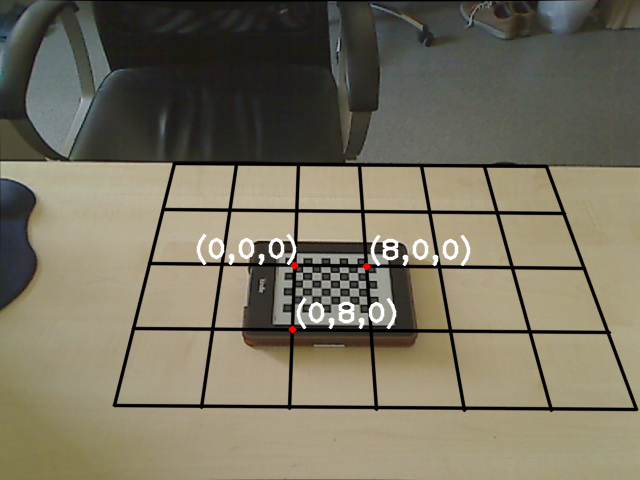
\includegraphics[width=205pt]{figures/pose0_180.png}
	\caption{Bal oldali kamera}
  \end{subfigure}
\begin{subfigure}[b]{.49\linewidth}
	\centering
	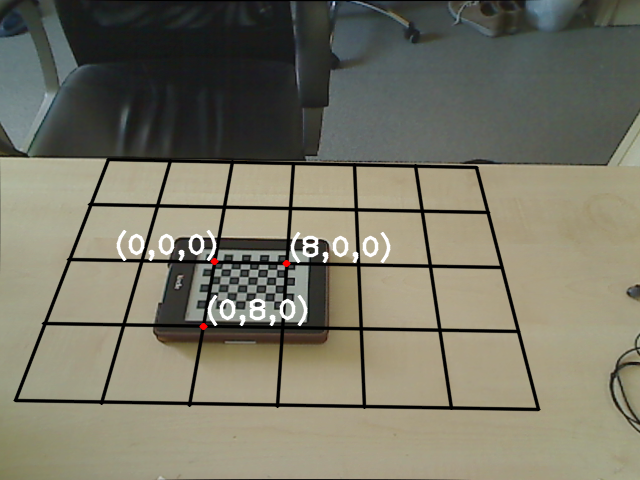
\includegraphics[width=205pt]{figures/pose1_180.png}
	\caption{Jobb oldali kamera}
  \end{subfigure}
\caption{Világ-koordinátarendszer jelölése a képeken \label{fig:pose}}
\end{figure}

%----------------------------------------------------------------------------
\section{Objektum detekció}
%----------------------------------------------------------------------------



\Aref{sec:obj_detection}. szekcióban leírtam a mozgó objektumok detekciójának egy lehetséges megközelítését. A lényege, hogy egy háttér modellt építünk, és így mindig aktuálisan lekérhető az előtérhez tartozó maszk, ami kijelöli a mozgó objektumokat. A probléma megoldása két fázisra bontható: először egyetlen objektumot keresek és detektálok, majd később több mozgó objektumot is.

Mindkét fázisnak közös része a már említett modellépítés, melyhez az OpenCV-ben megtalálható \texttt{BackgroundSubtractorMOG2} osztályt \cite{opencv-mog} hívom segítségül. Példányosítás után a modell építése, és az aktuális maszk kinyerése az \texttt{apply} metódussal történik. \Aref{fig:my_mog2}. ábrán látható a kinyerhető maszkra egy példa.

\begin{figure}[tbh]
\centering
\begin{subfigure}[b]{.32\linewidth}
	\centering
	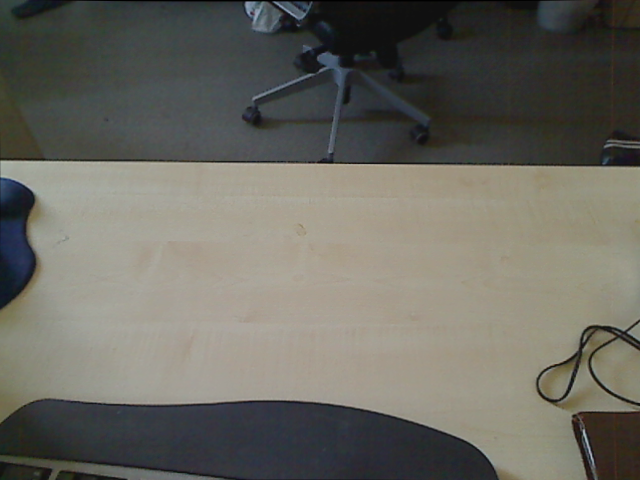
\includegraphics[width=137pt]{figures/image230.png}
	\caption{Statikus kép -- ,,háttér''}
  \end{subfigure}
\begin{subfigure}[b]{.32\linewidth}
	\centering
	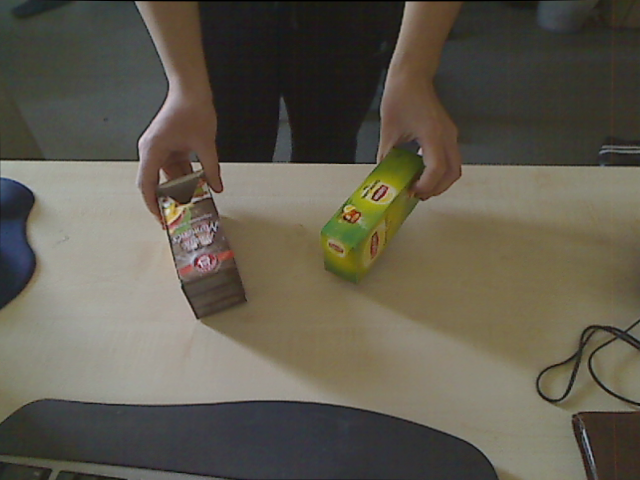
\includegraphics[width=137pt]{figures/image343.png}
	\caption{Mozgó képsor egy képe}
  \end{subfigure}
\begin{subfigure}[b]{.32\linewidth}
	\centering
	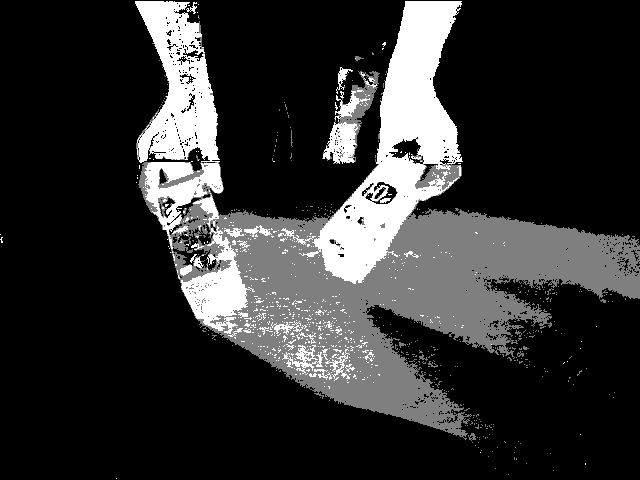
\includegraphics[width=137pt]{figures/mask343.png}
	\caption{Kapott előtér maszk}
  \end{subfigure}
\caption{Példa az előtér maszkra \label{fig:my_mog2}}
\end{figure}

Megfigyelhető, hogy a maszk nem pusztán bináris, hanem azt is jelzi, amit az algoritmus árnyéknak gondol. A zajt a maszkon az erózió-dilatáció morfológiai módszerek segítségével tudjuk csökkenteni. Előbbi a kisméretű zajokat tünteti el, utóbbi pedig a lyukakat szünteti meg. OpenCV-ben ezek implementációi a \texttt{dilate} és \texttt{erode} függvények. Előbbi az adott pixelt a környezetében (amit egy kernel ír le) lévő maximális, míg utóbbi a minimális értékkel helyettesít. Én egy erózió-dilatáció-erózió lépéssorozatot használok: először az apróbb szemcsék szűnnek meg, utána a lyukak. Az utolsó erózió szerepe, hogy az objektumok szélén a dilatáció miatt jelentkező növekedést megszűntesse. Ennek eredménye látható \aref{fig:erosion_dilation}. ábrán.

\begin{figure}[tbh]
\centering
\begin{subfigure}[b]{.49\linewidth}
	\centering
	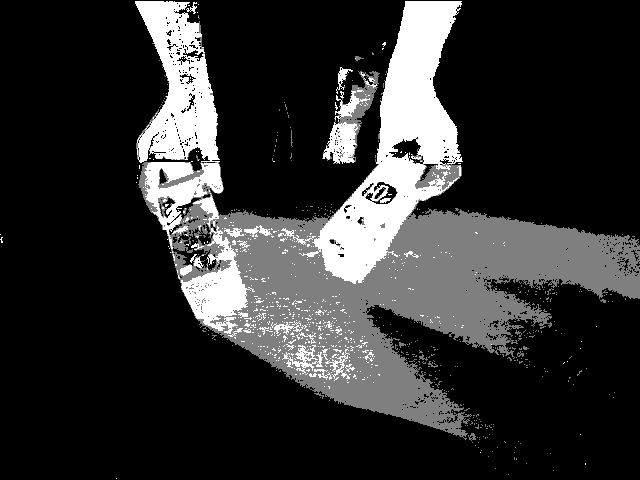
\includegraphics[width=205pt]{figures/mask343.png}
	\caption{Eredeti}
  \end{subfigure}
\begin{subfigure}[b]{.49\linewidth}
	\centering
	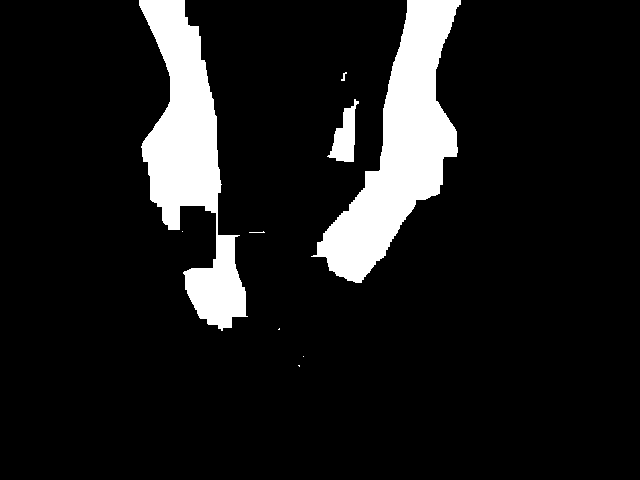
\includegraphics[width=205pt]{figures/mask343_fixed.png}
	\caption{Árnyékok kivétele és zajcsökkentés után}
  \end{subfigure}
\caption{Előtér maszk zajmentesítése \label{fig:erosion_dilation}}
\end{figure}

Megfigyelhető, hogy a bal oldali dobozhoz tartozó maszk része annyira zajos volt, hogy a nagy lyuk nem szűnt meg, míg a kevésbé zajos jobb oldali doboz rendben megmaradt. A maszkot alkalmazva az eredeti képre \aref{fig:mask_applied}. ábrán látható, hogy egy bizonyos hibahatáron belül sikeresnek tekinthető a mozgó részlet kijelölése.

\begin{figure}[tbh]
\centering
\begin{subfigure}[b]{.49\linewidth}
	\centering
	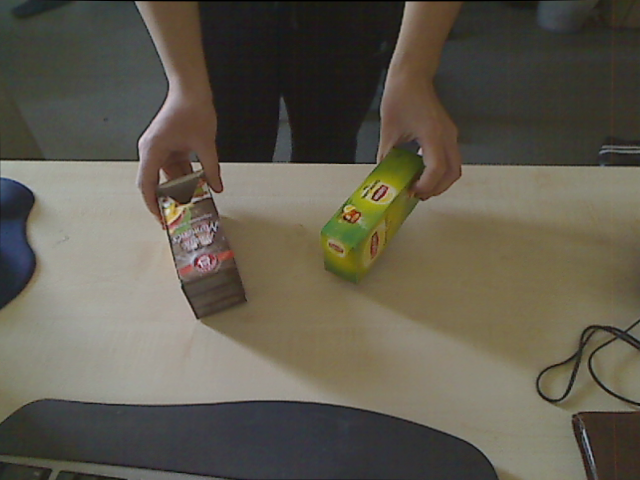
\includegraphics[width=205pt]{figures/image343.png}
	\caption{Eredeti kép}
  \end{subfigure}
\begin{subfigure}[b]{.49\linewidth}
	\centering
	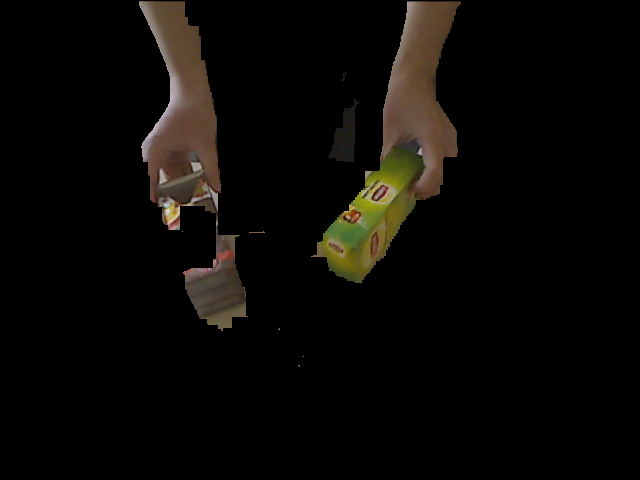
\includegraphics[width=205pt]{figures/mask343_applied.png}
	\caption{A detektált előtér}
  \end{subfigure}
\caption{Előtér maszk alkalmazás az eredeti képre \label{fig:mask_applied}}
\end{figure}

\subsection{Egyetlen objektum detekciója}

Kezdetben azzal az egyszerűsítéssel élek, hogy a képen csak egyetlen mozgó objektumot detektálok, mégpedig azt, amelyik a legnagyobb részt foglalja el a képen. Ez nagyban egyszerűsíti a dolgokat, mert ahogy majd látni fogjuk a következő szekcióban, az optikai folyam meghatározására szükség lesz a képeken látható \textit{blob}ok (egy objektumhoz tartozó egybefüggő rész a képen) párosításra a kamerák képein. Mivel összesen egy blobot jelölök ki a képeken, ezek párosítása triviális, és nagy valószínűséggel ugyanazon objektumhoz tartoznak majd.

Ezen logikát egy \texttt{SingleObjectSelector} osztályban implementáltam. Egyetlen metódusa van, amely paraméterül a képet és a (zajcsökkentett) előtér maszkot várja, visszatérési értéke pedig a kép azon része, melyet a maszk legnagyobb területű blobja jelöl ki. Ez utóbbit a \texttt{lastMask}-ban le is lehet kérdezni, és a későbbi könnyebb feldolgozás érdekében az ehhez tartozó befoglaló téglalapot is (\texttt{lastBoundingRect}). A megoldásom az OpenCV \texttt{findContours()} függvényére épít. Segítségével lekérem a maszkon található legkülső kontúrokat (a belső lyukakat is az objektum részének tekintem), és ezek közül azt választom, amelyiknek a legnagyobb a területe (ehhez a \texttt{cv::contourArea()}-t hívom segítségül).

\begin{figure}[tbh]
\centering

\begin{tikzpicture} 

\begin{class}[text width=10 cm]{SingleObjectSelector}{0, 0}
\attribute{+ lastMask : Mat}
\attribute{+ lastBoundingRect : Rect}

\operation{+ selectUsingContourWithMaxArea(img, mask) : Mat}
\end{class}

\end{tikzpicture}

\caption{\texttt{SingleObjectSelector} osztály \label{fig:cd:singleobjectselector}}
\end{figure}

\Aref{fig:maxArea}. ábrán látható az előbbiekben bemutatott maszkhoz meghatározott kontúrok és teli fehérrel a kiválasztott legnagyobb blob.

\begin{figure}[tbh]
    \centering
    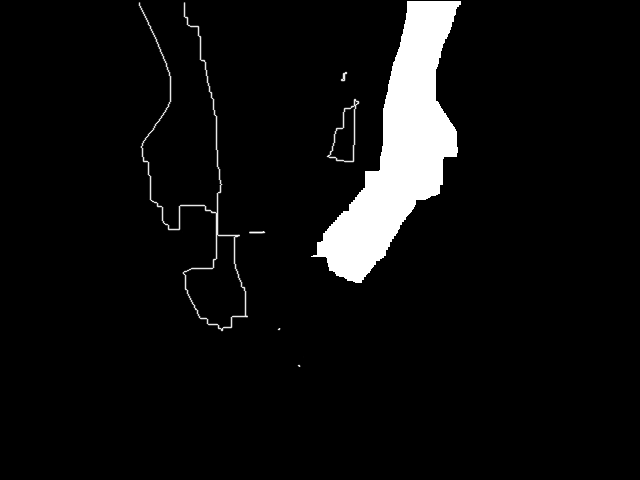
\includegraphics[width=250pt]{figures/mask343_contours.png}
    \caption{Legnagyobb blob kijelölése \label{fig:maxArea}}
\end{figure}

\subsection{Több objektum detekciója, párosítás a kamerák képein}

{\color{red} TODO...}



%----------------------------------------------------------------------------
\section{Optikai folyam meghatározása}
%----------------------------------------------------------------------------


\Aref{chapter2}. fejezetben bemutattam a sűrű optikai folyamok meghatározására Gunner Farnebäck módszerét. Ennek alkalmazását, valamint OpenCV-ben történő implementációjáról lesz szó ebben a részben.

A \texttt{cv::calcOpticalFlowFarneback()} függvény segítségével két képkockán meghatározhatom az optikai folyamot. Az algoritmus jellegéből adódóan nagy mozgásokat nem tud követni, de az implementáció támogatja a piramis-módszert, azaz nagy mozgások esetén a képeket több lépcsőben kicsinyíti, így az eredeti képen lévő nagy mozgások kisebbek lesznek, a kicsik pedig eltűnnek. A futási idő természetesen függ a kép méretétől, így fontos, hogy kihasználjuk az objektum maszkjából nyerhető információt.

A következőkben \aref{fig:of_original}. ábrán látható két képkocka lesz a kiinduló állapot, már az előbbiekben bemutatott előtér maszk által kijelölve. A képkockák két olyan kamera beállításal készültek, ahol a két kamera képsíkja nagyjából egybe esik (egy irányba néznek), és csak víszintes irányban vannak egymáshoz képest eltolva.

\begin{figure}[tbh]
\centering
\begin{subfigure}[b]{.49\linewidth}
	\centering
	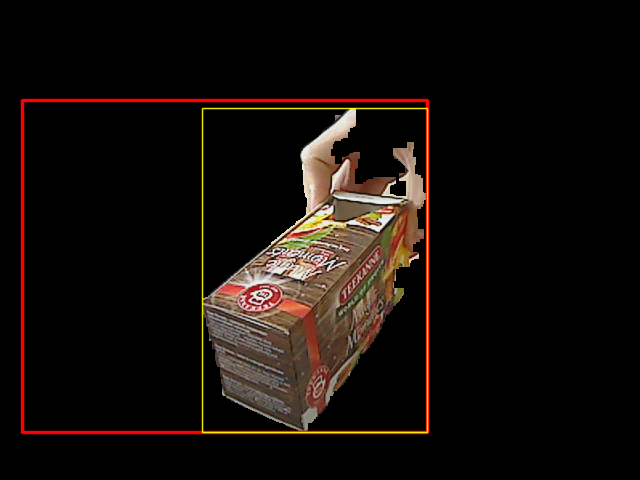
\includegraphics[width=205pt]{figures/of_img_left_framed.png}
  \end{subfigure}
\begin{subfigure}[b]{.49\linewidth}
	\centering
	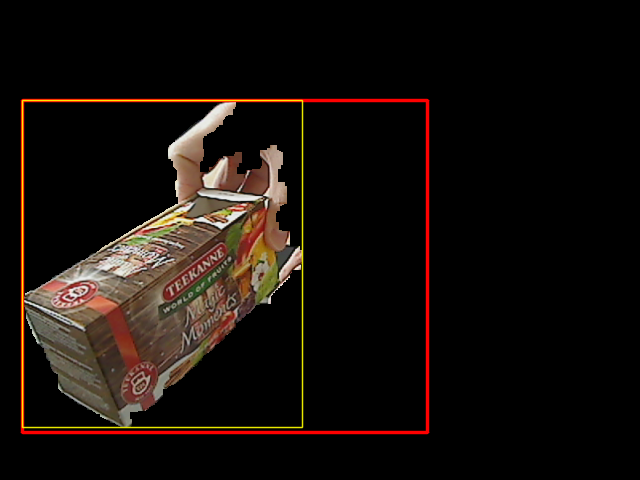
\includegraphics[width=205pt]{figures/of_img_right_framed.png}
  \end{subfigure}
\caption{Bal és jobb kamera által látott objektum kijelölve; a sárga keretek jelölik az objektumok befoglaló téglalapjait, a piros pedig ezen téglalapokat tartalmazó legkisebb területű téglalapot \label{fig:of_original}}
\end{figure}

Első megközelítésem, hogy a két objektum befoglaló téglalapját tekintem, és veszem azt a téglalapot, mely a legkisebb területű azok közül, amely mindkettőt tartalmazza. Kivágva ezt a téglalapot a két képből, két egyforma méretű képrészletet kapok, melyek külön-külön tartalmazzák a teljes objektumot. Ez látható \aref{fig:of_original}. ábrán pirossal jelölve. Erre a két részletre számolva optikai folyamot, 7 646 darab vektort kaptam, melyek közül néhányat vizualizáltam \aref{fig:bad0}. ábrán. A vektorok kezdő és végpontjaiból alkotok pontpárokat, ezeket tekintem egymásnak megfelelő pontoknak a két képen. Jól látható, hogy a kevés kirajzolt pontpárból egyik sem tekinthető jónak, mert a doboz különböző lapjaihoz tartozó pontok. Ez a nagy elmozdulás miatt van, hiába a piramis módszer, nem használható a végeredmény.

\begin{figure}[tbh]
\centering
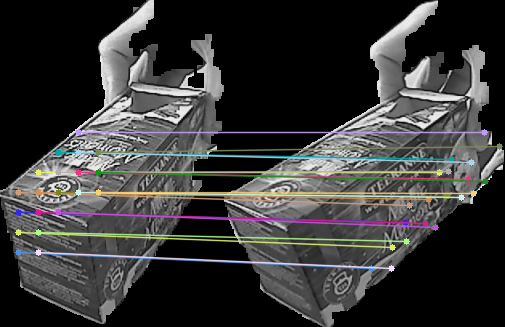
\includegraphics[width=300pt]{figures/vis_bad_0.png}
\caption{Első megközelítés (36 958 vektor) \label{fig:bad0}}
\end{figure}

A következő lépésem, hogy a két képet az egész kép közepére mozgatom, azaz a befoglaló téglalapok középpontja egybeesik. Ettől azt várom, hogy a valóságban egymásnak megfelelő pontok közelebb kerülnek egymáshoz, és így nagyobb eséllyel lesz valós a kiszámolt megfeleltetés. Ez 36 958 vektort eredményezett, melyeknek egy része \aref{fig:bad1}. ábrán látható. A találatok között még mindig akad szemmel láthatóan nem jó párosítás.

\begin{figure}[tbh]
\centering
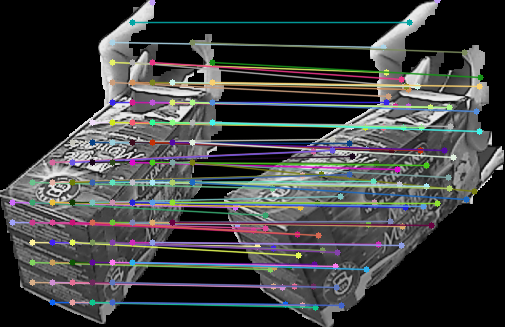
\includegraphics[width=300pt]{figures/vis_bad_1.png}
\caption{Közös középpontba mozgatás után (36 958 vektor) \label{fig:bad1}}
\end{figure}

Legyen két képkocka $K_1$ és $K_2$, valamint $F_{1, 2} = \mathcal{F}(K_1, K_2)$ és $F_{2, 1} = \mathcal{F}(K_2, K_1)$, ahol $\mathcal{F}$ jelöli két képkocka közti optikai-folyam operátort, melynek eredménye egy vektormező ($F_{1, 2}, F_{2, 1} : \mathbb{R}^2 \rightarrow \mathbb{R}^2$). A párosítást minőségét, pontosságát javítja ha megkövetelem, hogy ha $x\in K_1$ és $F_{1,2}(x) = v$, akkor $$



esetén optikai folyamot számolunk $F_1$-ből $F_2$-be, és egy $x\in F_1$ képponthoz tartozó vektor $v$, azaz $x + v = x' \in F_2$, akkor az $F_2$-ből $F_1$-be számolt optikai folyam esetén $x' \in F_2$ képponthoz tartozó $v'$ vektor esetén: $x' + v' \approx x \in F_1$.

%----------------------------------------------------------------------------
\section{Háromszögelés}
%----------------------------------------------------------------------------


%----------------------------------------------------------------------------
\section{Párhuzamosítás, több-szálúsítás}
%----------------------------------------------------------------------------


%----------------------------------------------------------------------------
\section{Eredmények, mérések, értékelés {\color{red} külön fejezet?}}
%----------------------------------------------------------------------------

